\documentclass{beamer}

\usepackage{graphicx}
\usepackage{hyperref}
\usepackage{listings}
\usepackage{tikz}

% beamer configuration
\mode<presentation> {
	\usetheme{Hannover}
}
\setbeamercolor{block title}{bg=yellow!50,fg=black}
\setbeamercolor{block body}{bg=yellow!10,fg=black}
\setbeamercovered{transparent}
\setbeamertemplate{frametitle}[default][left]
\AtBeginSection[]{
	\begin{frame}
		\vfill
		\centering
		\begin{beamercolorbox}[center]{title}
			\usebeamerfont{title}\insertsectionhead\par%
		\end{beamercolorbox}
		\vfill
	\end{frame}
}

% listings configuration
\lstset{
	basicstyle=\footnotesize,
	showstringspaces=false
}

% tikz configuration
\tikzset{
	reg/.style = {
		shape=rectangle,
		draw,
		align=left,
		top color=blue!10,
		bottom color=blue!10
	}
}





\title[]{An Introduction to Developing Web Applications with Flask}

\subtitle{\vspace{0.25in} 
\includegraphics[scale=.15]{images/flask-logo.png}}

\author[]{Prudhvi Boyapalli}

\institute{Hack \& Learn 2017 Workshop \\ Rice Computer Science Club}

\date{}

\begin{document}

\begin{frame}
	\titlepage
\end{frame}

\begin{frame}[t]{}
	\tableofcontents
\end{frame}

\section{Introduction}

\subsection{Flask}
	\begin{frame}[t]{How does a web app work? What does Flask do?}
		Flask is a Python microframework for building web applications.

		\begin{center}
		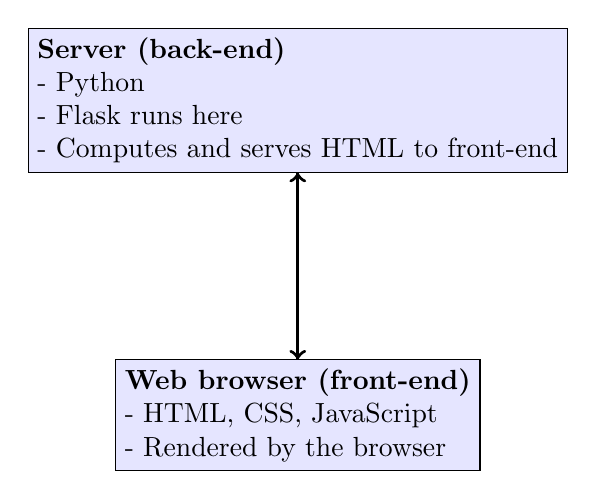
\begin{tikzpicture}
		\node[reg] (server) at (0,0) {
			\textbf{Server (back-end)}\\
			- Python\\
			- Flask runs here\\
			- Computes and serves HTML to front-end
		};
		\node[reg] (browser) at (0, -4) {
			\textbf{Web browser (front-end)}\\
			- HTML, CSS, JavaScript\\
			- Rendered by the browser
		};
		\draw[very thick, ->] (server) -- (browser);
		\draw[very thick, ->] (browser) -- (server);
		\end{tikzpicture}
		\end{center}
	\end{frame}


\subsection{Setup}
	\begin{frame}[t]{Install Python}
		\begin{itemize}
			\item{Basic level of Python knowledge is needed for this tutorial}
			\begin{itemize}
				\item{If you've taken COMP140 you're in good shape}
			\end{itemize}

			\item{Install Python if you haven't already: \url{python.org}}

			\item{I'm using 2.7, Flask also supports 3.3+}
		\end{itemize}
	\end{frame}


	\begin{frame}[t]{Install Flask}
		\begin{itemize}
			\item{
				Install Flask using PIP
				\begin{itemize}
					\item{\textbf{P}ip \textbf{I}nstalls \textbf{P}ackages from
						the \textbf{Py}thon \textbf{P}ackage \textbf{I}ndex a.k.a. PyPI}
				\end{itemize}
			}
		\end{itemize}

		\begin{block}{Flask Installation}
		\begin{semiverbatim}
			> sudo pip install Flask
		\end{semiverbatim}
		\end{block}
	\end{frame}


	\begin{frame}[t]{Editing}
		An IDE is overkill for this workshop. Use a programmer's editor that
		you're comfortable with:
		\begin{itemize}
			\item{Vim (All platforms)}
			\item{Atom (All platforms)}
			\item{Visual Studio Code (All platforms)}
			\item{Sublime Text (All platforms)}
			\item{Notepad++ (Windows)}
			\item{TextMate (OSX)}
			\item{Whatever floats your boat}
		\end{itemize}
	\end{frame}


	\begin{frame}[t]{Debugging}
		You'll be testing and debugging your code from the browser, so use one
		with good developer tools:
		\begin{itemize}
			\item{Chrome}
			\item{Firefox}
		\end{itemize}

		Other browsers can be used, but Chrome or Firefox will minimize the
		chance of running into browser specific issues.
	\end{frame}


\section{Hello World}

\subsection{Basic Example}
	\begin{frame}[t]{Super basic hello world example}
		This is the bare minimum code needed on the back-end to serve a web
		page
		\begin{block}{./code/hello\_world\_example/hello\_world.py}
			\lstinputlisting[language=Python]{../code/hello_world_example/hello_world.py}
		\end{block}
	\end{frame}


	\begin{frame}[t]{Running the web app}
		Once we've written the flask code, we can run the server locally and
		view the results in our web browser

		\begin{block}{Execute these commands to run the code:}
			\begin{semiverbatim}
				> cd /directory/with/project

				> export FLASK\_APP=hello\_world.py

				> flask run
			\end{semiverbatim}
		\end{block}\pause

		\begin{block}{Then you'll see something like:}
			\begin{semiverbatim}
				* Serving Flask app "hello\_world"

				* Running on \url{http://127.0.0.1:5000/}

					(Press CTRL+C to quit)
			\end{semiverbatim}
		\end{block}
	\end{frame}

\subsection{Closer Look}
	\begin{frame}[t]{How did that work?}
		\begin{enumerate}
			\item{We started up a local flask server which is listening at
					IP address 127.0.0.1, port 5000}
			\pause
			\item{We visited this page and the browser sent a request to our
					flask server}
			\pause
			\item{Because we visited \url{127.0.0.1:5000/} (emphasis on the
					\texttt{"/"}), the method bound to \texttt{"/"} was invoked}
			\pause
			\item{The \texttt{hello()} method in \texttt{hello\_world.py} was
					executed and the return value is sent to the browser as
					HTML}
			\pause
			\item{The browser received the HTML and rendered the webpage}
		\end{enumerate}
	\end{frame}


\subsection{Variable Routing}
	\begin{frame}[t]{Interactive hello world with variable routing}
		Now that we have a basic idea of how flask works, we can do some cool
		stuff with routing:
		\begin{block}{./code/hello\_world\_example/hello\_user.py}
			\lstinputlisting[language=Python]{../code/hello_world_example/hello_user.py}
		\end{block}
	\end{frame}

	\begin{frame}[t]{Running the new and improved web app}
		\begin{block}{As before:}
			\begin{semiverbatim}
				> export FLASK\_APP=hello\_user.py

				> flask run

				* Serving Flask app "hello\_world"

				* Running on \url{http://127.0.0.1:5000/}

					(Press CTRL+C to quit)
			\end{semiverbatim}
		\end{block}

		\begin{block}{Hello World}
			\url{http://127.0.0.1:5000/world}
		\end{block}
		\begin{block}{Hello $<$user$>$}
			\url{http://127.0.0.1:5000/user/Foo}

			\url{http://127.0.0.1:5000/user/Bar}
		\end{block}
	\end{frame}

\section{TODO: Complete Web App}

\subsection{Project Structure}
% TODO

\subsection{HTTP Communication}
% TODO

\subsection{Putting It All Together}
% TODO


\section{Conclusion}

\subsection{Summary}
	\begin{frame}[t]{Summary \& Next Steps}
		We covered:
		\begin{itemize}
			\item{Basic routing}
			\item{Accessing request data}
			\item{\texttt{GET} and \texttt{POST} requests}
			\item{Building and serving a complex web app with HTML, CSS and
					JavaScript}
		\end{itemize}
	\end{frame}


	\begin{frame}[t]{Next Steps}
		\begin{block}{More Flask Features}
			\begin{itemize}
				\item{URL Building}
				\item{Additional HTTP Methods (\texttt{GET, POST, DELETE,} etc.)}
				\item{HTML templates with placeholders}
				\item{User file uploads}
				\item{Reading and writing cookies}
				\item{Redirects and error handling}
				\item{Managing sessions}
			\end{itemize}
		\end{block}

		\begin{block}{Deploying your web app}
			Once you've developed and tested you app locally, you can deploy
			your flask code and make it publicly accessible. There lots of
			tutorials on how to do this for various cloud providers (AWS,
			Azure, DigitalOcean, etc).
		\end{block}
	\end{frame}


\subsection{Resources}
	\begin{frame}[t]{Resources}
		\begin{itemize}
			\item{
				\textbf{This presentation \& and all of the code}\\
				\indent \url{github.com/hack-rice/flask-tutorial}
			}
			\item{
				\textbf{Flask website \& awesome documentation}\\
				\indent \url{flask.pocoo.org}
			}
		\end{itemize}
	\end{frame}

	\begin{frame}[t]{Contact}
		Prudhvi Boyapalli
		\begin{itemize}
			\item{prb2 AT rice.edu}
		\end{itemize}

		HackRice
		\begin{itemize}
			\item{Fall 2017}
			\item{Annual hackathon right here on campus}
			\item{Great way to hone your skills and make something cool}
		\end{itemize}

		RiceApps
		\begin{itemize}
			\item{Work on a team of students to build useful applications}
			\item{Great way to gain hands on development experience}
			\item{\url{http://riceapps.org}}
		\end{itemize}

		Rice CS Facebook Group
		\begin{itemize}
			\item{\url{https://facebook.com/groups/365985373415471}}
		\end{itemize}

		CS Club Facebook Page
		\begin{itemize}
			\item{\url{https://facebook.com/ricecsclub}}
		\end{itemize}
	\end{frame}

\end{document}
